% ============================================================================
%  Capítulo 1 — Introducción
% ============================================================================
\chapter{Introducción}
\label{cap:introduccion}

La gestión integral de los recursos hídricos se ha consolidado como un pilar
fundamental para garantizar la sostenibilidad ambiental y el bienestar social
frente al deterioro ecológico actual. En este contexto, el tratamiento y la
reutilización de aguas residuales no solo alivian la presión sobre las fuentes
de agua dulce, sino que son acciones directas para el cumplimiento de los
Objetivos de Desarrollo Sostenible (ODS), específicamente el ODS~6, que
garantiza agua limpia y saneamiento, y el ODS~11, enfocado en ciudades
sostenibles. Ahora bien, las Plantas de Tratamiento de Aguas Residuales (PTAR)
juegan un rol protagónico en este ciclo, permitiendo la recuperación del
recurso para su reintegración segura al medio ambiente o su aprovechamiento en
sectores productivos \cite{un2015sdg,khalid2018review}.

Dentro de la operación de una PTAR, específicamente en el proceso de lodos
activados, la concentración de oxígeno disuelto (OD) es uno de los parámetros
críticos. Un nivel adecuado de OD es indispensable para el equilibrio
microbiológico y la degradación de materia orgánica, con un valor de
referencia de 2,0~mg/L. Sin embargo,
su dinámica es altamente no lineal y con múltiples variaciones debido a factores
como el clima, el caudal de entrada y la carga orgánica, o a factores de
operación como el ruido en las señales de medida, la activación de sopladores
auxiliares y los retardos propios del sistema. Por ende, mantener este
parámetro dentro del rango operativo es vital, ya que una baja concentración
compromete la calidad del efluente, mientras que una aireación excesiva
representa un desperdicio energético considerable; de modo que una mala
regulación reúne a la vez el riesgo ambiental y elevados costos energéticos en
el proceso \cite{wei2020disturbance,amand2013review}.

A nivel industrial, la estrategia predominante para la regulación del OD sigue
siendo el control Proporcional-Integral-Derivativo (PID), debido a su
simplicidad y familiaridad operativa: se entiende, se mantiene y se sintoniza
sin detener la planta. No obstante, los controladores PID convencionales
presentan limitaciones estructurales significativas al enfrentar las fuertes no
linealidades, las perturbaciones inherentes al proceso e incluso las señales
ruidosas propias de los ambientes industriales. Ahora bien, para el caso de
estudio de la PTAR, se evidencia que, según el estado de la planta, su ganancia
puede variar, lo que presenta dificultades a la hora de sintonizar y, en
algunos casos, un esfuerzo excesivo sobre la señal de control. Es decir, estas
deficiencias obligan a una sintonización conservadora que resulta en respuestas
lentas ante picos de carga o en una sobre-aireación constante por seguridad, lo
cual incrementa la ineficiencia energética y en algunos casos dificulta el
cumplimiento estricto de la normatividad ambiental
\cite{iratni2019advances,qiao2016self}.

Frente a estas barreras, el Control de Rechazo Activo de Perturbaciones (ADRC)
emerge como una solución robusta capaz de estimar y cancelar las perturbaciones
internas y externas mediante un Observador de Estado Extendido (ESO), sin
requerir un modelo matemático exacto de la planta. La idea se presenta de una
forma lineal y sintonizable, en la que no se intenta modelar cada perturbación por separado, sino estimarlo
todo en una única señal, la \emph{perturbación total}, y cancelarla de forma
aditiva. Lo más relevante
para la aplicación práctica es que avances recientes han permitido formular el
ADRC bajo arquitecturas equivalentes a los controladores PID industriales
estándar (1DOF/2DOF) o basadas en el error, facilitando su migración segura y
\emph{plug-and-play} en Controladores Lógicos Programables (PLC) comerciales,
superando así la brecha entre la teoría de control avanzado y la
implementación industrial
\cite{gao2014centrality,stankovic2024pid,madonski2019general}.

Bajo este marco, el presente proyecto se centra en el diseño, implementación y
validación de dos estrategias de control avanzado basadas en rechazo activo de
perturbaciones: un controlador proporcional-integral generalizado (GPI) y un
ADRC con ESO, ambos escritos sobre el error de seguimiento, para la regulación
de oxígeno disuelto en una planta de tratamiento de aguas residuales. Los dos
se enfrentan al mismo PID ISA de referencia con filtro en la acción derivativa,
a la misma perturbación, obtenida y sintetizada a partir de los datos reales de la planta. La investigación busca demostrar que estas técnicas no solo
pueden mejorar el desempeño transitorio, con una sintonización más sencilla y
un menor movimiento de la señal de control que el PID convencional, sino que también son viables técnicamente para ser embebidas en
la infraestructura de automatización existente, contribuyendo de esta forma a
la investigación de técnicas de
control emergentes que aún no son comunes a nivel industrial
\cite{wei2022scalable,Sangregorio2023}.

\section{Justificación}
\label{sec:justificacion}

El proyecto se fundamenta en evidenciar la posibilidad de utilizar un
paradigma de control diferente, como el ADRC, en entornos industriales. A pesar
de sus ventajas teóricas y de su creciente estudio académico, su adopción
industrial aún es reducida, y su implementación en PTAR es escasa
\cite{Wei2020b,wei2022scalable,Sangregorio2023}. Ahora bien, el lazo de control
de oxígeno disuelto en la etapa de lodos activados aparece como una
problemática en la que puede implementarse: muchas instalaciones operan con
controladores PID convencionales ajustados empíricamente, que presentan
limitaciones ante perturbaciones, variaciones de carga y caudal, ruido en las
señales y no linealidades del proceso biológico, lo que afecta la calidad del
efluente e incrementa el consumo energético en la aireación
\cite{khalid2018review,shen2009mpc,qiao2018adaptive}. Por tanto, evaluar el
ADRC en este lazo, bajo condiciones reales de operación, con variabilidad de
carga e instrumentación limitada, permite validar su desempeño y su grado de
robustez frente a la estrategia convencional.

Este proyecto se justifica en su contribución técnica por introducir una estrategia de
control avanzada con alto potencial de replicabilidad. Además, su
carácter innovador radica en llevar técnicas de control avanzado como el ADRC
desde el ámbito teórico hacia una implementación práctica, como caso de
estudio en un proceso de tratamiento de aguas residuales, generando evidencia a
partir de datos reales y abriendo camino para futuras aplicaciones
industriales \cite{amand2013review,santin2016advanced}.

\section{Antecedentes y estado del arte}
\label{sec:estado_arte}

\subsection{Control del oxígeno disuelto en PTAR}

Existen varios modelos estandarizados de una PTAR; esta investigación adopta
el \textit{Benchmark Simulation Model} n.\textsuperscript{o}~1 (BSM1),
desarrollado en el marco de la IWA, solo como guía
\cite{copp2002bsm1,alex2008bsm1}. Este entorno es el estándar para la
evaluación comparativa de estrategias de control, porque captura las no
linealidades y los acoplamientos hidráulicos típicos de un proceso de lodos
activados real \cite{wei2020disturbance}.

El BSM1 se divide en un biorreactor de cinco compartimientos, dos anóxicos y tres aerobios, y un
clarificador secundario, con recirculación interna de nitratos y externa de lodos; el clarificador se
modela en diez capas según Takács \cite{takacs1991settler}, y la biología según el ASM1
\cite{henze1987asm1}. En este documento, al igual que en la PTAR del caso de estudio, solo se tiene en
cuenta el tanque de aireación (tanque 5 del BSM1).

\subsubsection*{Dinámica del oxígeno disuelto en el tanque 5}

Siguiendo a Wei et al. \cite{wei2020disturbance} y la descripción del BSM1
\cite{alex2008bsm1}, el balance de oxígeno en el quinto compartimiento es

\begin{equation}
    \frac{dS_{O,5}}{dt} = \frac{1}{V_{5}}
    \left( Q_{4}S_{O,4} + r_{Z,5}V_5 + \KLa V_{5}\,(S_{O}^{*} - \SOc)
    - Q_{5}\SOc \right),
    \label{eq:intro_do}
\end{equation}

donde $r_{Z,5}$ es la tasa neta de consumo de oxígeno por la biomasa, que en el BSM1 se calcula con
el ASM1 \cite{henze1987asm1}. La Tabla~\ref{tab:intro_variables} recoge el significado de las
variables.

\begin{table}[H]
\centering
\caption{Variables del balance de oxígeno del tanque 5.}
\label{tab:intro_variables}
\renewcommand{\arraystretch}{1.25}
\small
\begin{tabular}{|c|p{8.6cm}|c|}
\hline
\rowcolor[gray]{0.9}
\textbf{Símbolo} & \textbf{Descripción} & \textbf{Unidad} \\ \hline
$\SOc$, $S_{O,4}$ & Oxígeno disuelto en los tanques 5 y 4 (salida controlada) & g~O$_2$/m$^3$ \\ \hline
$\KLa$ & Coeficiente de transferencia de oxígeno del tanque 5 (variable manipulada) & d$^{-1}$ \\ \hline
$Q_4$, $Q_5$ & Caudal que entra y sale del tanque 5 & m$^3$/d \\ \hline
$V_5$ & Volumen del tanque 5 & m$^3$ \\ \hline
$S_O^{*}$ & Concentración de saturación de oxígeno & g~O$_2$/m$^3$ \\ \hline
$r_{Z,5}$ & Tasa neta de consumo de oxígeno por la biomasa & g~O$_2$/(m$^3$\,d) \\ \hline
\end{tabular}
\end{table}

La ecuación de la dinámica servirá solo como guía, para identificar las perturbaciones que pueden
afectar el lazo de control y para analizar la estimación de la perturbación total realizada mediante el
observador de estado extendido; su desarrollo para la planta del caso de estudio está en la
Sección~\ref{sec:car_modelo}.

\subsection{Limitaciones del control convencional}

A pesar de décadas de avances teóricos, el PID sigue dominando el sector
industrial. Iratni y Chang \cite{iratni2019advances} señalan que su
ubicuidad se debe a la familiaridad de los operadores y a la facilidad de
mantenimiento. Qiao et al. \cite{qiao2016self} argumentan, sin embargo, que el
PID sufre limitaciones estructurales severas en el contexto de un proceso bioquímico: al ser un
controlador lineal de parámetros fijos, no puede adaptarse a las variaciones
de carga orgánica y caudal. Por ende, esto obliga a sintonizarlo de forma conservadora,
lo que produce respuesta lenta ante picos de carga (riesgo ambiental) o
sobre-aireación permanente para mantener margen (ineficiencia energética)
\cite{wei2020disturbance}.

El Capítulo~\ref{cap:caracterizacion} añade a ese diagnóstico general una
evidencia local y cuantitativa: en la planta estudiada, la ganancia incremental
del lazo varía entre ventanas, es decir, cada vez que se trate de hacer una identificación
práctica se pueden obtener diferentes valores en sus parámetros. Y un PID de
parámetros fijos puede parecer que está mal sintonizado; está sintonizado para un punto de un
rango que la planta recorre y varía todos los días, por lo que requiere una resintonización cada vez.



\subsection{Rechazo activo de perturbaciones}

Frente a estas limitaciones, el ADRC combina la simplicidad estructural del
PID con la robustez del control moderno. Propuesto por Han \cite{han2009adrc} y
formalizado en su versión lineal y parametrizada por ancho de banda por Gao
\cite{gao2003scaling,gao2014centrality}, no requiere un modelo detallado de la
planta: su núcleo es el ESO, que estima en tiempo real la perturbación total
que aquí incluye la respiración $r_{Z,5}$, las variaciones de caudal, el
error de modelado  y la cancela en la ley de control, creando una ley de control linealizante. Wei et al.
\cite{wei2020disturbance,Wei2020b} validaron el enfoque sobre el BSM1,
reportando reducción del IAE frente al PID y mejor eficiencia energética al reducir el esfuerzo sobre la señal de control. Herbst \cite{herbst2013practical} y Madoński y Herman
\cite{madonski2015survey} sistematizaron los aspectos prácticos (elección de
$\bo$, sintonía por ancho de banda, efecto del ruido y del retardo), y el
libro de Herbst y Madoński \cite{herbst2024adrc} recoge la formulación discreta
del ESO y su manejo de saturación. Para el GPI, el manejo de saturación se
toma del esquema de realimentación de la saturación del \emph{Control
Handbook} \cite{levine2011handbook}, tal como lo aplican Vargas-Medina et al.
\cite{vargas2026microgrids} al comparar el ADRC con un GPI robusto. Ambos
esquemas de manejo de saturación se usan en el diseño de los controladores.

La idea central se resume en la forma canónica del ADRC: todo lo que el
control no conoce se agrupa en una sola señal $\bar{\xi}$, la perturbación total, que
entra a la planta sumada a la entrada de control,

\begin{equation}
    y^{(n)}(t) = b_0\, u(t) + \bar{\xi}(t) ,
    \label{eq:intro_canonica}
\end{equation}

de modo que la planta, vista desde $u$, es una cadena de $n$ integradores
(Figura~\ref{fig:cadena_integradores}). Como $u$ y $\bar{\xi}$ entran por el mismo
punto, si se conoce $\bar{\xi}$
basta con restarla en $u$ para que la planta se comporte como los integradores
puros; rechazar la perturbación consiste, por
tanto, en estimar $\bar{\xi}$ y cancelarla antes de que llegue a la salida. Con la
estimación $\hat{\bar{\xi}}$ que entrega el ESO, la ley de control linealizante es

\begin{equation}
    u(t) = \frac{v(t) - \hat{\bar{\xi}}(t)}{b_0}
    \qquad\Longrightarrow\qquad
    y^{(n)}(t) = v(t) + \big(\bar{\xi}(t) - \hat{\bar{\xi}}(t)\big) \;\approx\; u_0(t) ,
    \label{eq:intro_linealizante}
\end{equation}

donde $v$ es una nueva entrada virtual. Si la estimación es buena, el error
$\bar{\xi}-\hat{\bar{\xi}}$ es pequeño y la planta, queda reducida a
$n$ integradores puros, que se controlan con una simple realimentación de
estados.

\subsubsection*{ADRC basado en el error}

En la forma clásica, el ESO necesita por separado la salida $y$ y la
referencia $r$. Por otro lado, los bloques de control industriales, en cambio, solo
reciben el error de seguimiento, igual que un PID. Herbst y Madoński
\cite{herbst2024adrc} muestran que el ADRC puede reescribirse para que el
observador trabaje directamente sobre el error $e = y - r$, como se ve en la
Figura~\ref{fig:adrc} del Capítulo~\ref{cap:ADRC-ESO} (Se aclara que Herbst y Madoński toman el error al contrario, $e = r - y$, pero en las secciones de diseño se tomará como $e = y - r$, es decir, con la referencia negativa).

El funcionamiento se explica de la siguiente forma: el ESO recibe el error $e$ y la señal de control
realmente aplicada $u_{\text{lim}}$ (después del limitador), y con ellas
estima el estado del error $\hat{\boldsymbol{x}}$, cuyo último elemento es la
perturbación total. La ganancia $\boldsymbol{l}$ corrige la estimación con la
diferencia entre el error medido y el estimado, $e - \boldsymbol{c}^{\top}
\hat{\boldsymbol{x}}$. Después, la realimentación
$(\boldsymbol{k}^{\top}\;1)\,\hat{\boldsymbol{x}}$ calcula la acción que lleva
el error a cero y cancela la perturbación estimada, y el bloque $1/\bo$ la
convierte en la señal física $u$. Como el observador se alimenta con
$u_{\text{lim}}$, la saturación del actuador no hace que la estimación se
desvíe, es decir que este tipo de controlador ya viene con un manejo de saturación incorporado, un anti-windup natural. 

\subsection{Control GPI (A Flat Filtering Approach)}

La escuela de control por planitud diferencial llega a un resultado
estructuralmente cercano por otro camino: el control proporcional-integral
generalizado (GPI) de Fliess et al. \cite{fliess2002gpi}, desarrollado para
sistemas planos por Sira-Ramírez et al. \cite{sira2017adrc}, sustituye el
observador asintótico por integrales iteradas del error, y modela la
perturbación como un polinomio de grado $m$ localmente válido. El resultado es
un controlador de una sola pieza, sin estados de observador explícitos, cuya
robustez proviene del mismo mecanismo y el rechazo de perturbaciones corresponde
a un modelo interno de la perturbación.

Sira-Ramírez et al. \cite[\S3.4.3]{sira2017adrc} presentan este enfoque, de
\emph{filtrado plano}, sobre el sistema de segundo orden no perturbado

\begin{equation}
    \ddot{F}(t) = u(t) ,
    \label{eq:sira_planta}
\end{equation}

donde $F$ es la salida plana y se desea que siga asintóticamente una
referencia suave $F^{*}(t)$. La entrada nominal es
$u^{*}(t) = \ddot{F}^{*}(t)$, y los errores de seguimiento de la salida y de
la entrada se definen como

\begin{equation}
    e_F(t) = F(t) - F^{*}(t), \qquad e_u(t) = u(t) - u^{*}(t).
    \label{eq:sira_errores}
\end{equation}

El control GPI elimina la necesidad de observadores asintóticos de estado
mediante \emph{reconstructores integrales}, que solo involucran la entrada y
la salida. En este caso, el reconstructor integral de $\dot{e}_F$ es

\begin{equation}
    \hat{\dot{e}}_F(t) = \int_0^t e_u(\sigma)\,d\sigma,
    \qquad
    \dot{e}_F(t) = \hat{\dot{e}}_F(t) + \dot{e}_F(0).
    \label{eq:sira_reconstructor}
\end{equation}

Incorporar este estimado en una realimentación lineal hace que la ley quede
afectada por valores constantes, como la condición inicial desconocida
$\dot{e}_F(0)$ y las perturbaciones externas. Para corregir ese efecto
desestabilizante se compensa con integraciones del error de la salida plana, y
se propone el controlador

\begin{equation}
    e_u(t) = -k_3\!\int_0^t\! e_u(\sigma)\,d\sigma
          - k_2\, e_F(t)
          - k_1\!\int_0^t\! e_F(\sigma)\,d\sigma
          - k_0\!\int_0^t\!\!\int_0^{\tau}\! e_F(\sigma)\,d\sigma\,d\tau ,
    \label{eq:sira_gpi}
\end{equation}

donde los coeficientes $\{k_3,k_2,k_1,k_0\}$ se eligen de modo que el
polinomio característico de lazo cerrado

\begin{equation}
    p(s) = s^{4} + k_3 s^{3} + k_2 s^{2} + k_1 s + k_0
    \label{eq:sira_polinomio}
\end{equation}

tenga todas sus raíces en el semiplano izquierdo. Aplicando la transformada de
Laplace a \eqref{eq:sira_gpi} se obtiene el controlador como una red de
compensación de adelanto,

\begin{equation}
    e_u(s) = -\,\frac{k_2 s^{2} + k_1 s + k_0}{s\,(s + k_3)}\; e_F(s) ,
    \label{eq:sira_tf}
\end{equation}

en la que el polo en el origen es el integrador que rechaza las
perturbaciones constantes y el factor $1/(s+k_3)$ proviene del reconstructor
integral. Toda la estructura se construye solo con integradores de la entrada
y del error, sin derivadas de la salida ni observador.

Rojas y Cortés-Romero \cite{rojas2020equivalence} demuestran, en el dominio
de la frecuencia, que el observador GPI, en sus versiones de orden completo y
de orden reducido, y como caso particular el ESO, es equivalente a un
observador de perturbación clásico con un filtro $Q(s)$ de estructura
específica. A partir de esa equivalencia analizan cómo influyen en la robustez
y el desempeño el orden del sistema, el número de estados extendidos, la
incertidumbre en la ganancia de control y el método de sintonía. Además,
recopilan las equivalencias ya conocidas entre el ADRC y otras estructuras,
como los filtros planos y el PID. Siguiendo la línea de la equivalencia entre
el ADRC y los filtros planos, en este trabajo se busca la correspondencia entre el GPI construido con
reconstructores integrales y el ADRC con ESO, es decir, el cambio de
ganancias de $(\wc,\wo)$ a $(k_0,k_1,k_2)$. Ambas son formas
equivalentes que solo difieren en su implementación y en el manejo de la
saturación, y se explora cómo integrar las dos estructuras en un solo bloque de
PLC que pueda configurarse como cualquiera de ellas.

\subsection{Integración industrial}

Una barrera histórica para la adopción de control avanzado ha sido la
dificultad de trasladar algoritmos académicos a un PLC. La literatura reciente
propone tres soluciones que este trabajo utiliza directamente.

\textbf{Equivalencia formal y migración segura.} Stankovi\'c et al.
\cite{stankovic2024pid} demuestran que un ADRC lineal puede reescribirse en la
forma estándar de un controlador industrial de uno o dos grados de libertad, de
modo que es posible diseñar un ADRC que, en su configuración inicial, se
comporte exactamente igual que el PID ya instalado, y luego aumentar
progresivamente el ancho de banda del observador sin riesgo operativo
(Figura~\ref{fig:pid2adrc}).

\begin{figure}[H]
    \centering
    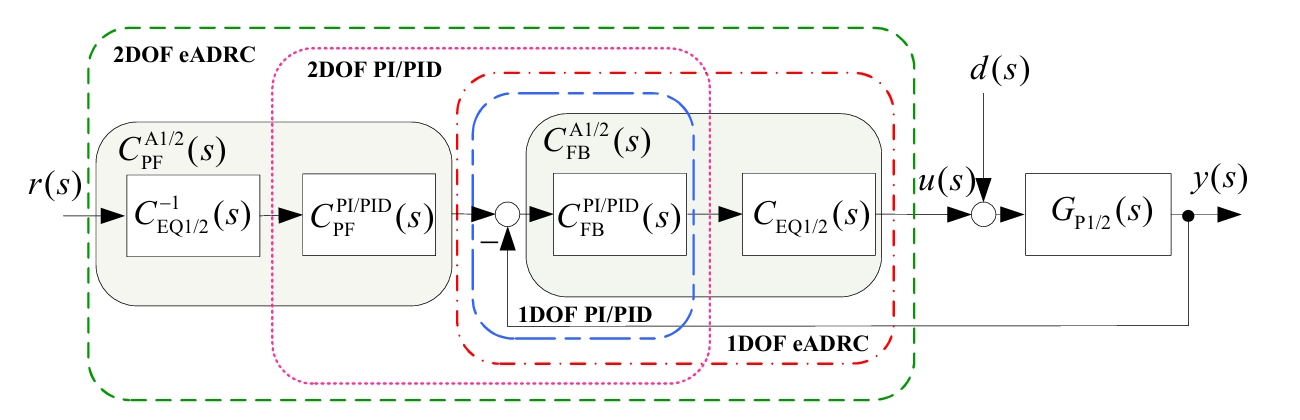
\includegraphics[width=0.95\linewidth]{pid2adrc.png}
    \caption[Equivalencias PID--eADRC]{Esquema de implementación de
    controladores PI/PID y eADRC en configuraciones 1DOF y 2DOF, y su
    equivalencia para plantas de orden relativo 1 y 2
    \cite{stankovic2024pid}.}
    \label{fig:pid2adrc}
\end{figure}

\textbf{ADRC basado en el error.} La mayoría de los algoritmos ADRC requieren
acceso independiente a $y$ y a $u$. Madoński et al. \cite{madonski2019general}
observan que muchos bloques de control comerciales tienen arquitectura cerrada
y solo aceptan el error $e=r-y$, y proponen el \emph{general error-based ADRC},
que reformula el ESO para depender exclusivamente del error de seguimiento.
Ese es el esquema que se implementa aquí, y es la razón por la que el bloque
resultante puede sustituir al PID existente sin recablear el lazo.

\textbf{Sintonía en el dominio de la frecuencia.} Cao et al.
\cite{cao2025cascaded} reinterpretan el ADRC como un PID precedido por filtros
en cascada (Figura~\ref{fig:casc}), lo que permite aplicar márgenes de ganancia
y de fase para ajustar sus parámetros y razonar sobre el compromiso entre
atenuación de ruido de sonda y velocidad de recuperación ante carga --- que en
este trabajo resulta ser, cuantitativamente, el compromiso que decide el
diseño.

\begin{figure}[H]
    \centering
    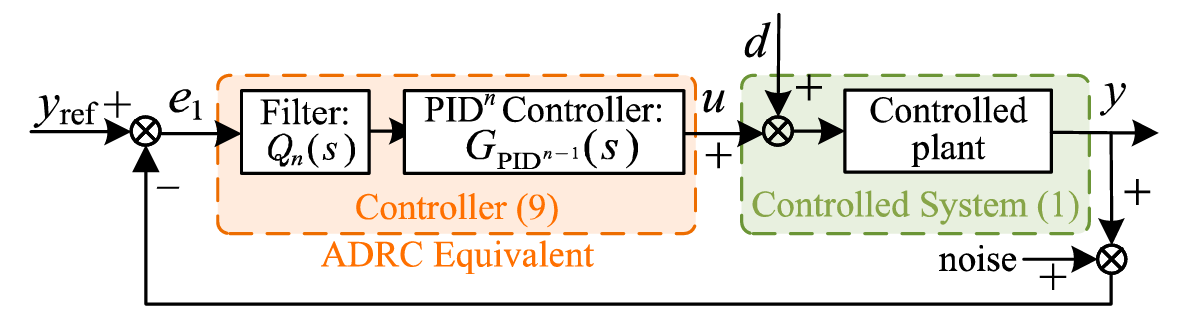
\includegraphics[width=0.72\linewidth]{casc.png}
    \caption[ADRC en forma de PID con filtro en cascada]{Esquema eADRC
    implementado en su forma equivalente de PID con filtro en cascada
    \cite{cao2025cascaded}.}
    \label{fig:casc}
\end{figure}

\subsection{Análisis comparativo}

La Tabla~\ref{tab:comparativa_control} sintetiza las fortalezas y debilidades
identificadas en la revisión, y fundamenta la elección del ADRC como estrategia
central.

\begin{table}[H]
\centering
\caption{Comparación técnica de estrategias de control para lodos activados.}
\label{tab:comparativa_control}
\renewcommand{\arraystretch}{1.35}
\small
\begin{tabular}{|p{2.1cm}|p{4.6cm}|p{4.9cm}|p{2.6cm}|}
\hline
\rowcolor[gray]{0.9}
\textbf{Estrategia} & \textbf{Ventajas} & \textbf{Limitaciones} & \textbf{Referencia} \\ \hline
\textbf{PID} & Estructura simple, bajo costo computacional, base instalada amplia. & No desacopla perturbaciones fuertes; compromiso entre rapidez y estabilidad; una sola sintonía para todo el rango de operación. & Iratni \& Chang \cite{iratni2019advances} \\ \hline
\textbf{MPC / NMPC} & Manejo explícito de restricciones y de sistemas multivariables. & Costo computacional elevado; sensible al error de modelo; mantenimiento difícil. & Li \& Yamamoto \cite{li2017multi} \\ \hline
\textbf{RN / Difuso} & Modela dinámicas complejas sin ecuaciones explícitas. & Estructura opaca; validación de estabilidad difícil; depende de datos de calidad. & Qiao et al. \cite{qiao2014neural} \\ \hline
\textbf{ADRC / GPI} & Estima y cancela la perturbación total; equilibrio entre desempeño y simplicidad; sintonía por ancho de banda. & Requiere diseño cuidadoso del observador ante ruido de medida; menor penetración comercial. & Wei et al. \cite{wei2020disturbance} \\ \hline
\end{tabular}
\end{table}

\subsection{Métricas de desempeño y robustez}
\label{subsec:metricas}

Para comparar los controladores a lo largo del documento se usan las métricas clásicas de desempeño y
de esfuerzo de control de la Tabla~\ref{tab:metricas}. Se miden desde el instante
$t_0$ del cambio de consigna o de la perturbación hasta el final de la ventana $t_f$, con el error de
seguimiento $e(t) = y(t) - r(t)$ y el tamaño del cambio de consigna $\Delta r$.

\begin{table}[H]
\centering
\caption{Métricas de desempeño y de esfuerzo de control usadas en el documento.}
\label{tab:metricas}
\small
\renewcommand{\arraystretch}{1.15}
\begin{tabular}{@{}l>{\centering\arraybackslash}p{6.0cm}>{\raggedright\arraybackslash}p{7.0cm}@{}}
\toprule
\textbf{Métrica} & \textbf{Definición} & \textbf{Qué mide} \\
\midrule
IAE & $\displaystyle\int_{t_0}^{t_f} |e(t)|\,dt$ & Error acumulado en la ventana. \\
$\overline{|e|}$ & $\dfrac{\mathrm{IAE}}{t_f - t_0}$ & Error absoluto medio; compara ventanas de distinta duración. \\
ITAE & $\displaystyle\int_{t_0}^{t_f} (t - t_0)\,|e(t)|\,dt$ & Error acumulado, pesando más el que tarda en desaparecer. \\
RMS & $\displaystyle\sqrt{\frac{1}{t_f - t_0}\int_{t_0}^{t_f} e^2(t)\,dt}$ & Error cuadrático medio. \\
$\max|e|$ & $\max_t\,|e(t)|$ & Mayor desviación; ante una perturbación, la caída máxima. \\
$M_p$ & $\dfrac{100\,\max_t\,\operatorname{sgn}(\Delta r)\,\bigl(y(t) - r\bigr)}{|\Delta r|}$ & Sobrepico, en \% del cambio de consigna; ante una perturbación, en \% de la caída máxima. \\
$t_s$ & menor $t_s$ con $|e(t)| \le 0{,}02\,|\Delta r|$ para todo $t \ge t_0 + t_s$ & Tiempo de asentamiento, con banda de $2~\%$ del cambio. \\
\midrule
$u_{\max}$, $u_{\min}$ & $\max_t\,u(t)$, \ $\min_t\,u(t)$ & Valores extremos de la señal de control. \\
$E_u$ & $\displaystyle\int_{t_0}^{t_f} \bigl(u(t) - u_\infty\bigr)^2\,dt$ & Energía de la señal de control respecto a su valor final. \\
TV & $\displaystyle\sum_k \bigl|u[k] - u[k-1]\bigr|$ & Variación total, el recorrido del actuador; TV/h, por hora. \\
$\sigma_u$ & $\operatorname{std}\bigl(u_{\text{con ruido}} - u_{\text{sin ruido}}\bigr)$ en estacionario & Ruido del sensor que llega a la señal de control. \\
$\sigma_{\Delta u}/\sqrt{2}$ & $\operatorname{std}\bigl(u[k] - u[k-1]\bigr)/\sqrt{2}$ & Movimiento de $u$ de una muestra a la siguiente. \\
\bottomrule
\end{tabular}
\end{table}

Para la robustez se usan las métricas clásicas de la Tabla~\ref{tab:metricas_robustez}, calculadas
sobre el lazo abierto $G_L(s) = C(s)\,G(s)$, con la planta $G(s)$ y el controlador $C(s)$;
$\omega_{gc}$ es el cruce de ganancia y $\omega_{pc}$, el cruce de fase.

\begin{table}[H]
\centering
\caption{Métricas de robustez usadas en el documento.}
\label{tab:metricas_robustez}
\small
\renewcommand{\arraystretch}{1.3}
\begin{tabular}{@{}l>{\centering\arraybackslash}p{6.0cm}>{\raggedright\arraybackslash}p{7.0cm}@{}}
\toprule
\textbf{Métrica} & \textbf{Definición} & \textbf{Qué mide} \\
\midrule
MF & $180^{\circ} + \angle G_L(j\omega_{gc})$, \newline con $|G_L(j\omega_{gc})| = 1$ & Margen de fase: la fase que puede perder el lazo antes de volverse inestable. \\
MG & $1/|G_L(j\omega_{pc})|$, \newline con $\angle G_L(j\omega_{pc}) = -180^{\circ}$ & Margen de ganancia: cuánto puede crecer la ganancia del lazo. \\
$\theta_{\max}$ & $\dfrac{\pi}{180^{\circ}}\,\dfrac{\mathrm{MF}}{\omega_{gc}}$ & Retardo máximo que aguanta el lazo. \\
$M_s$ & $\max_{\omega}\,|S(j\omega)|$, \newline con $S(s) = 1/\bigl(1 + G_L(s)\bigr)$ & Pico de la sensibilidad; entre más bajo, más robusto. \\
$M_t$ & $\max_{\omega}\,|T(j\omega)|$, \newline con $T(s) = G_L(s)/\bigl(1 + G_L(s)\bigr)$ & Pico de la sensibilidad complementaria; resonancia del lazo cerrado. \\
$\omega_{BW}$ & $|T(j\omega)| < 1/\sqrt{2}$ para $\omega > \omega_{BW}$ & Ancho de banda del lazo cerrado ($-3$~dB); qué tan rápido es el lazo. \\
\bottomrule
\end{tabular}
\end{table}

\section{Planteamiento del problema}
\label{sec:problema}

En la industria, la mayoría de los lazos de control se siguen cerrando con
controladores PID sintonizados de forma empírica, que al ser lineales y de
parámetros fijos solo quedan bien ajustados para un punto de operación. Esto
se vuelve una limitación en procesos no lineales, con múltiples perturbaciones
asociadas y múltiples incertidumbres, en los que se plantea la necesidad de un
cambio de paradigma: buscar nuevos controladores que dejen de lado el PID y
compitan directamente con él, en vista de una mejora en el desempeño y de un
avance tecnológico. El ADRC ofrece esa posibilidad, ya que permite implementar
un controlador lineal sobre un sistema no lineal, agrupando las perturbaciones
y las incertidumbres en una sola señal que se estima y se cancela en línea.

Ahora bien, un caso donde este paradigma puede implementarse es el lazo de
oxígeno disuelto en la etapa de lodos activados de una PTAR. Este proceso es
no lineal, incierto en algunos parámetros y está sometido a perturbaciones como el caudal de entrada, la carga
orgánica, la activación de sopladores y el ruido en las señales de medida, y
debe mantenerse en un rango de operación de 1,5 a 2,5~mg/L. Por ende, un PID
convencional ISA sintonizado empíricamente puede resultar en una regulación
imprecisa del OD y un consumo energético
ineficiente.  Es
decir, el problema no es solo mejorar la regulación del OD, sino demostrar que
algoritmos de control más avanzados pueden implementarse en un PLC, competir
directamente contra el PID y ofrecer algunas ventajas dadas por su estructura,
su forma de sintonización y su funcionamiento.


\section{Objetivos}
\label{sec:objetivos}

\subsection{Objetivo general}

Comparar dos estrategias de control basadas en rechazo activo de
perturbaciones para la regulación del oxígeno disuelto en la etapa de lodos
activados de una planta de tratamiento de aguas residuales, con el fin de
mejorar el desempeño frente a perturbaciones operativas como el caudal de
entrada, el ruido de los sensores de oxígeno, la activación de aireadores
auxiliares, y las asociadas a variaciones en la carga orgánica y en los
parámetros químicos del afluente.

\subsection{Objetivos específicos}

\begin{itemize}
  \item[\textbf{OE1}] Caracterizar las perturbaciones que afectan el sistema de
  dosificación de oxígeno en la etapa de lodos activados, con el propósito de
  apoyar el diseño y la evaluación de los controladores basados en rechazo
  activo de perturbaciones.
  \item[\textbf{OE2}] Diseñar un primer controlador proporcional-integral
  generalizado (GPI) robusto basado en el error de seguimiento para el proceso
  de dosificación de oxígeno.
  \item[\textbf{OE3}] Diseñar un segundo controlador con rechazo activo de
  perturbaciones basado en observador de estado extendido (ESO) enfocado en el
  error de seguimiento.
  \item[\textbf{OE4}] Desarrollar una metodología para la implementación de
  controladores basados en rechazo activo de perturbaciones en entornos
  industriales mediante PLC, considerando aspectos prácticos como el manejo de
  saturación y la facilidad de implementación.
  \item[\textbf{OE5}] Validar experimentalmente los controladores propuestos
  frente a un PID convencional, empleando métricas clásicas de desempeño y
  robustez.
\end{itemize}


\section{Metodología}
\label{sec:metodologia}

El trabajo se desarrolló en seis fases, cada una asociada a uno o varios capítulos del documento
y a los objetivos específicos (Tabla~\ref{tab:metodologia}).

\begin{table}[H]
\centering
\caption{Resumen de la metodología del trabajo.}
\label{tab:metodologia}
\renewcommand{\arraystretch}{1.08}
\small
\begin{tabular}{|p{1.2cm}|>{\raggedright\arraybackslash}p{2.9cm}|>{\raggedright\arraybackslash}p{10.1cm}|}
\hline
\rowcolor[gray]{0.9}
\textbf{Fase} & \textbf{Etapa} & \textbf{Descripción} \\ \hline
\textbf{Fase 1} & Revisión y caracterización (Cap.~\ref{cap:introduccion} y~\ref{cap:caracterizacion}; OE1) &
\textbullet~Estado del arte del control de OD, del ADRC y del GPI.\newline
\textbullet~Análisis de los datos de operación: régimen diario, lazo con el PID, escalones del soplador y caudales.\newline
\textbullet~Perturbación total reconstruida de los datos, su espectro y el ruido del sensor. \\ \hline
\textbf{Fase 2} & Modelado (Cap.~\ref{cap:caracterizacion}) &
\textbullet~Modelo de primer orden con retardo identificado de los escalones, con sus rangos de variación.\newline
\textbullet~Validación con los datos, planta nominal y ganancia $b_0$. \\ \hline
\textbf{Fase 3} & Diseño de controladores (Cap.~\ref{cap:ADRC-ESO} y~\ref{cap:GPI}; OE2 y OE3) &
\textbullet~ADRC con ESO basado en el error de seguimiento, con sintonía por anchos de banda.\newline
\textbullet~GPI con integradores y su equivalencia con el ADRC con ESO.\newline
\textbullet~Análisis de robustez y ante variaciones de la planta, en Python y Simulink. \\ \hline
\textbf{Fase 4} & Implementación en PLC (Cap.~\ref{cap:implementacion}; OE4) &
\textbullet~Saturación, acondicionamiento de la referencia, ruido y retardo.\newline
\textbullet~Discretización y realización con retardos.\newline
\textbullet~Bloques de función en texto estructurado, probados en el PLC con una planta simulada. \\ \hline
\textbf{Fase 5} & Validación (Cap.~\ref{cap:comparacion_pid}; OE5) &
\textbullet~Simulación contra un PID ISA de igual robustez: consigna, retardo, ruido y perturbación reconstruida.\newline
\textbullet~Métricas de desempeño (IAE, ITAE, sobrepico, tiempo de asentamiento) y de esfuerzo de control. \\ \hline
\textbf{Fase 6} & Análisis y documentación (Cap.~\ref{cap:discusion} y~\ref{cap:conclusiones}) &
\textbullet~Discusión de resultados, limitaciones e implicaciones prácticas.\newline
\textbullet~Recetas de implementación y redacción del documento. \\ \hline
\end{tabular}
\end{table}



